\documentclass[journal]{IEEEtran}

\usepackage{cite}
\usepackage{graphicx}
\usepackage{amsmath}
\usepackage{amssymb}
\usepackage{array}
\usepackage{multirow}
\usepackage{booktabs}
\usepackage{url}
\usepackage{hyperref}
\usepackage{color}
\usepackage{xcolor}
\usepackage{colortbl}
\usepackage{enumitem}
\usepackage{balance}

\definecolor{lightpurple}{HTML}{E8E0F0}

\hyphenation{op-tical net-works semi-conduc-tor}

\begin{document}

% ─────────────────────────────────────────────────────────────────────────────
\title{Evaluating LLMs for Grade-Aware and Child-Safe Educational
       Question Answering: A Controlled Ablation Study on ScienceQA}

\author{Ali~Saab,~\IEEEmembership{Student Member,~IEEE,}
        and~Nadine~Charaf,~\IEEEmembership{Student Member,~IEEE}
\thanks{A. Saab and N. Charaf are with the Department of Electrical
and Computer Engineering, Western University, London, ON, Canada.
E-mail: \{asaab9, ncharaf\}@uwo.ca. Submitted in partial fulfilment of
ECE 9660 -- Large Language and Vision Models.}}

\markboth{ECE 9660 Course Report,~Western University,~2025}%
{Saab and Charaf: LLMs for Grade-Aware Educational QA}

\maketitle

% ─────────────────────────────────────────────────────────────────────────────
\begin{abstract}
Large language models (LLMs) are increasingly deployed as tutoring
assistants for K--12 students. Yet most evaluations measure only answer
accuracy, ignoring whether responses are grounded in instructional material,
aligned with pedagogical hints, or calibrated to the student's grade level.
We present a systematic zero-shot ablation study on ScienceQA examining
how three contextual signals---lecture passages, pedagogical hints, and
grade-level metadata---individually and jointly affect five diverse LLMs
spanning 3\,B to 26\,B parameters. We define five prompt conditions (C0--C4)
that incrementally add each signal and evaluate 375 carefully filtered examples
across grades 3--7 (75 per grade). Our results show that (i) lecture text
alone \emph{decreases} accuracy for most local models, (ii) pedagogical hints
are the single most impactful signal with gains up to $+12.8$ percentage
points, (iii) grade metadata provides negligible accuracy gains but reduces
calibration error by 38\%, and (iv) Claude Haiku reaches 98.4\% accuracy
under the hint condition. We release prompt templates, evaluation code, and
results to support reproducible research in LLM-based educational systems.
\end{abstract}

\begin{IEEEkeywords}
Large language models, K--12 education, question answering, ablation study,
grade-aware prompting, ScienceQA, lecture grounding, pedagogical hints,
Ollama, zero-shot prompting.
\end{IEEEkeywords}

% ─────────────────────────────────────────────────────────────────────────────
\section{Introduction}
\label{sec:introduction}

The rapid adoption of LLMs in education has opened new possibilities for
personalised tutoring, instant feedback, and scalable instructional
support~\cite{kasneci2023chatgpt,holmes2019artificial}. Tools built on
models such as GPT-4 and Claude are already used by millions of students
for homework assistance and exam preparation~\cite{wardat2023chatgpt}.
However, the gap between benchmark accuracy and \emph{suitability for
K--12 deployment} remains poorly understood.

Educational use of LLMs imposes requirements beyond correctness. A model
serving a Grade~3 student should (i) ground its explanation in the provided
lecture; (ii) incorporate pedagogical hints when available; and (iii) produce
explanations whose vocabulary and sentence complexity match the student's
grade level. These dimensions---\emph{grounding}, \emph{hint alignment}, and
\emph{grade calibration}---are orthogonal to accuracy yet critical for
child-safe deployment. Despite their importance, prior evaluations focus
exclusively on answer accuracy~\cite{lu2022scienceqa}.

\textbf{Contributions:}
\begin{enumerate}[leftmargin=*, label=(\roman*)]
  \item A five-condition ablation framework (C0--C4) that isolates the
        effect of each contextual signal available in ScienceQA.
  \item A principled sampling strategy ensuring all 375 examples have all
        required fields and span grades 3--7 with exact balance (75 per
        grade, seed = 42).
  \item Zero-shot evaluation of five LLMs: Llama 3.2 3B, Phi-4 Mini,
        Llama 3.1 8B, Mixtral 8x7B, and Claude Haiku, covering open-weight
        local models and a commercial API.
  \item Seven evaluation metrics spanning accuracy, grounding, hint
        alignment, and grade calibration, revealing non-obvious interactions
        between model size, context type, and grade difficulty.
\end{enumerate}

% ─────────────────────────────────────────────────────────────────────────────
\section{Related Work}
\label{sec:related}

Lu et al.~\cite{lu2022scienceqa} introduced ScienceQA with multimodal
chain-of-thought for fine-tuned models; our work examines zero-shot
prompting of general-purpose LLMs with ablated contextual signals.
Retrieval-augmented generation~\cite{lewis2020rag} grounds responses in
retrieved documents, analogous to our C1--C4 lecture injection;
chain-of-thought prompting~\cite{wei2022chain} improves reasoning accuracy
but combines signals without isolating individual contributions.
Kochmar et al.~\cite{kochmar2022automated} demonstrated that personalised
feedback in intelligent tutoring systems improves student outcomes,
motivating our hint and grade conditioning study. Readability metrics such
as Flesch-Kincaid Grade Level~\cite{kincaid1975derivation} have long been
used to assess text complexity; applying them to evaluate LLM output
alignment with grade metadata is novel in the educational QA context.

% ─────────────────────────────────────────────────────────────────────────────
\section{Dataset and Sampling}
\label{sec:dataset}

\subsection{ScienceQA}

ScienceQA~\cite{lu2022scienceqa,thomas2024scienceqa} is a large-scale K--12
QA dataset of 21,208 multiple-choice questions spanning grades 1--12.
Each example optionally includes a lecture passage, pedagogical hint,
solution, optional image, and grade metadata. We use only the \textbf{test
split} (4,241 examples) to avoid training data leakage.

\subsection{Eligibility Filter and Stratified Sampling}

Table~\ref{tab:filter} shows the five-step eligibility pipeline. Our
experimental conditions require non-empty lecture, hint, grade, and solution
fields for every example simultaneously. The hint filter (Step~3) is the
most restrictive, reducing the pool by 64\% and concentrating examples in
elementary and middle-school science content.

\begin{table}[h]
\centering
\caption{Eligibility Filter Pipeline (ScienceQA Test Split)}
\label{tab:filter}
\renewcommand{\arraystretch}{1.25}
\begin{tabular}{clrr}
\toprule
\textbf{Step} & \textbf{Filter} & \textbf{Remaining} & \textbf{\%} \\
\midrule
0 & Full test split   & 4,241 & 100.0 \\
\rowcolor{lightpurple}
1 & No image          & 2,224 &  52.4 \\
2 & Has lecture       & 2,152 &  50.7 \\
\rowcolor{lightpurple}
3 & Has hint          &   778 &  18.3 \\
4 & Has grade         &   778 &  18.3 \\
\rowcolor{lightpurple}
5 & Has solution      &   602 &  14.2 \\
\midrule
  & \textbf{Eligible} & \textbf{602} & \textbf{14.2} \\
\bottomrule
\end{tabular}
\end{table}

Of the 602 eligible examples, only grades 3--7 have at least 75 examples
each (grades 1--2 lack formal lecture passages; grades 10--12 are almost
entirely image-based; grades 8--9 fall below the 75-example threshold).
We draw 75 examples per grade via stratified random sampling (seed = 42),
yielding $N = 375$. This balanced design ensures per-grade accuracy
comparisons are not confounded by sample size differences.

% ─────────────────────────────────────────────────────────────────────────────
\section{Experimental Design}
\label{sec:method}

\subsection{Prompt Conditions (C0--C4)}

Table~\ref{tab:conditions} defines five conditions as a factorial ablation
over three binary contextual signals. The condition pairs C0/C1, C1/C2,
C1/C3, and C0/C4 isolate the lecture, hint, grade, and total context
effects. All prompts use zero-shot instruction following with temperature
0.0 and a 300-token output limit. The C4 template begins with a grade-aware
system preamble (``You are a science tutor for a [GRADE] student. Use
simple, age-appropriate language.''), followed by the lecture passage,
the pedagogical hint, the question, and the labelled choices. Lower
conditions omit their respective fields; C0 provides only the question
and choices, establishing a pure parametric-knowledge baseline.

\begin{table}[h]
\centering
\caption{Five Prompt Conditions: Ablation Over Contextual Signals}
\label{tab:conditions}
\renewcommand{\arraystretch}{1.3}
\begin{tabular}{clccc}
\toprule
\textbf{ID} & \textbf{Description} & \textbf{Lecture} & \textbf{Hint} & \textbf{Grade} \\
\midrule
\rowcolor{lightpurple}
C0 & Question Only (No Context) & --         & --         & -- \\
C1 & + Lecture                  & \checkmark & --         & -- \\
\rowcolor{lightpurple}
C2 & + Lecture + Hint           & \checkmark & \checkmark & -- \\
C3 & + Lecture + Grade          & \checkmark & --         & \checkmark \\
\rowcolor{lightpurple}
C4 & Full Context               & \checkmark & \checkmark & \checkmark \\
\bottomrule
\end{tabular}
\end{table}

\subsection{Research Questions}

\begin{itemize}[leftmargin=*]
  \item \textbf{RQ0}: How accurately do LLMs answer K--12 science questions
        with no context? (C0 baseline)
  \item \textbf{RQ1}: Does a lecture passage improve accuracy? (C0 $\to$ C1)
  \item \textbf{RQ2}: Does a pedagogical hint improve accuracy? (C1 $\to$ C2)
  \item \textbf{RQ3}: Does grade metadata improve accuracy or language
        calibration? (C1 $\to$ C3)
\end{itemize}

% ─────────────────────────────────────────────────────────────────────────────
\section{Evaluation Metrics}
\label{sec:metrics}

We define seven metrics in three groups that together operationalise
\emph{educational suitability}, not merely factual correctness.

\textbf{(1) Accuracy Metrics.}
\emph{Answer Accuracy} is $\text{Acc} = \frac{1}{N}\sum_i \mathbf{1}[\hat{a}_i = a_i^*]$,
where $a_i^*$ is the ground-truth answer and $\hat{a}_i$ is the first capital
letter matching a valid choice in the response (unparseable responses are
marked incorrect).
\emph{Choice Consistency} $\text{Cons} = \frac{1}{N}\sum_i \mathbf{1}[\hat{a}_i \neq \varnothing]$
measures instruction-following reliability independently of correctness.
\emph{Per-Grade Accuracy} $\text{Acc}_g$ is computed over the 75 balanced
examples for each $g \in \{3,\ldots,7\}$.

\textbf{(2) Grounding and Alignment Metrics.}
\emph{Lecture Grounding Semantic} (LG-Sem) is the cosine similarity between
sentence-transformer embeddings~\cite{reimers2019sbert}
(\texttt{all-MiniLM-L6-v2}) of the model response and the lecture passage.
\emph{Lecture Grounding Overlap} (LG-Ovlp) is the ROUGE-1
recall~\cite{lin2004rouge} of lecture content words in the response, i.e.,
the fraction of lecture vocabulary reused by the model.
\emph{Hint Alignment Semantic} (HA-Sem) and \emph{Hint Alignment Overlap}
(HA-Ovlp) apply the same two measures to the hint text. Since hints are
shorter (1--2 sentences) and more targeted than lectures (2--5 sentences),
HA-Ovlp is a tighter signal of whether the model anchors on the specific
pedagogical concept.

\textbf{(3) Calibration Metrics.}
\emph{Grade Calibration Error} is:
\begin{equation}
  \bar{e} = \frac{1}{N}\sum_{i=1}^{N}\bigl|\,\text{FKGL}(r_i) - g_i^*\,\bigr|,
  \label{eq:calib}
\end{equation}
where $\text{FKGL}(r_i)$ is the Flesch-Kincaid Grade Level~\cite{kincaid1975derivation}
of model response $r_i$, computed as
$0.39\cdot(W/S) + 11.8\cdot(Y/W) - 15.59$
($W$ = words, $S$ = sentences, $Y$ = syllables), and $g_i^* \in \{3,\ldots,7\}$
is the target grade. Lower $\bar{e}$ indicates responses that are
linguistically appropriate for the intended audience.

% ─────────────────────────────────────────────────────────────────────────────
\section{Models}
\label{sec:models}

\begin{table}[h]
\centering
\caption{LLMs Evaluated in This Study}
\label{tab:models}
\renewcommand{\arraystretch}{1.25}
\begin{tabular}{llll}
\toprule
\textbf{Model} & \textbf{Params} & \textbf{Architecture} & \textbf{Deploy} \\
\midrule
\rowcolor{lightpurple}
Llama 3.2 3B~\cite{llama32}     & 3B   & LLaMA 3.2 dense & Ollama \\
Phi-4 Mini~\cite{phi4}          & 3.8B & Phi-4 dense     & Ollama \\
\rowcolor{lightpurple}
Llama 3.1 8B~\cite{llama31}     & 8B   & LLaMA 3.1 dense & Ollama \\
Mixtral 8x7B~\cite{mixtral}     & 47B  & Mixtral MoE     & Ollama \\
\rowcolor{lightpurple}
Claude Haiku~\cite{claudehaiku} & --   & Anthropic Claude & API   \\
\bottomrule
\end{tabular}
\end{table}

Local models are served via Ollama~\cite{ollama} using instruct-tuned chat
variants, ensuring reproducibility without API costs. Mixtral 8x7B is a
mixture-of-experts model with $\sim$13B active parameters per token,
providing near-70B-class quality while remaining tractable for local
inference. Claude Haiku (\texttt{claude-haiku-4-5-20251001}) serves as a
strong closed-source reference representing the upper bound of production
educational API quality.

% ─────────────────────────────────────────────────────────────────────────────
\section{Results}
\label{sec:results}

\subsection{Overall Accuracy}

Table~\ref{tab:main} reports accuracy and choice consistency for all models
across all conditions ($N = 375$ per cell).

\begin{table*}[t]
\centering
\caption{Overall Accuracy (\%) and Choice Consistency (\%) by Model and Condition.
         $\Delta$ columns show absolute change vs.\ C0 baseline.}
\label{tab:main}
\renewcommand{\arraystretch}{1.35}
\begin{tabular}{lcccccccccc}
\toprule
& \multicolumn{2}{c}{\textbf{C0 No Context}}
& \multicolumn{2}{c}{\textbf{C1 Lecture}}
& \multicolumn{2}{c}{\textbf{C2 +Hint}}
& \multicolumn{2}{c}{\textbf{C3 +Grade}}
& \multicolumn{2}{c}{\textbf{C4 Full}} \\
\cmidrule(lr){2-3}\cmidrule(lr){4-5}\cmidrule(lr){6-7}\cmidrule(lr){8-9}\cmidrule(lr){10-11}
\textbf{Model} & Acc & Cons & Acc & $\Delta$ & Acc & $\Delta$ & Acc & $\Delta$ & Acc & $\Delta$ \\
\midrule
\rowcolor{lightpurple}
Llama 3.2 3B  & 76.8 & 100.0 & 68.8 & $-8.0$   & 74.9 & $-1.9$   & 69.3 & $-7.5$ & 75.7 & $-1.1$  \\
Phi-4 Mini    & 66.1 & 100.0 & 67.2 & $+1.1$   & 77.6 & $+11.5$  & 67.2 & $+1.1$ & 77.1 & $+11.0$ \\
\rowcolor{lightpurple}
Llama 3.1 8B  & 88.8 & 100.0 & 81.3 & $-7.5$   & 88.8 & $\pm0.0$ & 82.1 & $-6.7$ & 89.9 & $+1.1$  \\
Mixtral 8x7B  & 83.5 &  98.9 & 81.6 & $-1.9$   & 90.4 & $+6.9$   & 81.6 & $-1.9$ & 91.2 & $+7.7$  \\
\rowcolor{lightpurple}
Claude Haiku  & 85.6 &  89.9 & 89.1 & $+3.5$   & 98.4 & $+12.8$  & 88.8 & $+3.2$ & 98.1 & $+12.5$ \\
\midrule
\textbf{Average} & 80.2 & 97.8 & 77.6 & $-2.6$ & 86.0 & $+5.9$  & 77.8 & $-2.4$ & 86.4 & $+6.3$  \\
\bottomrule
\end{tabular}
\end{table*}

\textbf{C0 baseline (RQ0).} Accuracy spans 66.1\% (Phi-4 Mini) to 88.8\%
(Llama 3.1 8B), confirming substantial parametric science knowledge. The
high C0 floor for Llama 3.1 8B and Claude Haiku limits headroom for
context-based improvements.

\textbf{Lecture effect (RQ1).} Adding the lecture \emph{reduces} accuracy for
three of five models: Llama 3.2 3B ($-8.0$~pp), Llama 3.1 8B ($-7.5$~pp),
and Mixtral ($-1.9$~pp). Only Phi-4 Mini ($+1.1$~pp) and Claude Haiku
($+3.5$~pp) benefit. We term this the \emph{grounded but distracted} effect:
models read the lecture but anchor on passages irrelevant to the specific question.

\textbf{Hint effect (RQ2).} Hints are the dominant signal. Every model shows
substantial C1$\to$C2 gains: Claude Haiku $+9.3$~pp, Phi-4 Mini $+10.4$~pp,
Mixtral $+8.8$~pp, Llama 3.1 8B $+7.5$~pp. Hints act as an attentional cue,
directing models toward the relevant concept within the lecture.

\textbf{Grade metadata (RQ3).} Grade alone has negligible accuracy impact
($\leq$3~pp). This is expected---grade metadata shapes language register, not
answer selection. Its calibration effect is examined in
Section~\ref{sec:calib}.

\subsection{Accuracy Heatmap and Condition Trends}

\begin{figure}[t]
\centering
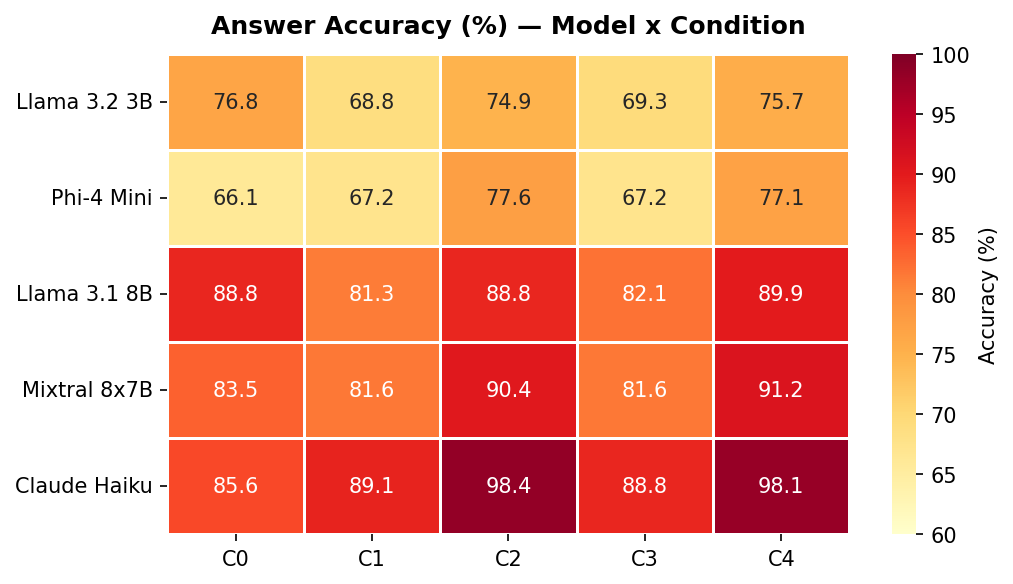
\includegraphics[width=\columnwidth]{Fig/fig1_accuracy_heatmap.png}
\caption{Accuracy (\%) across all model $\times$ condition combinations.
The warm stripe at C2/C4 confirms the dominant hint effect; the cool
stripe at C1/C3 shows lecture and grade alone are insufficient for local models.}
\label{fig:heatmap}
\end{figure}

\begin{figure*}[t]
\centering
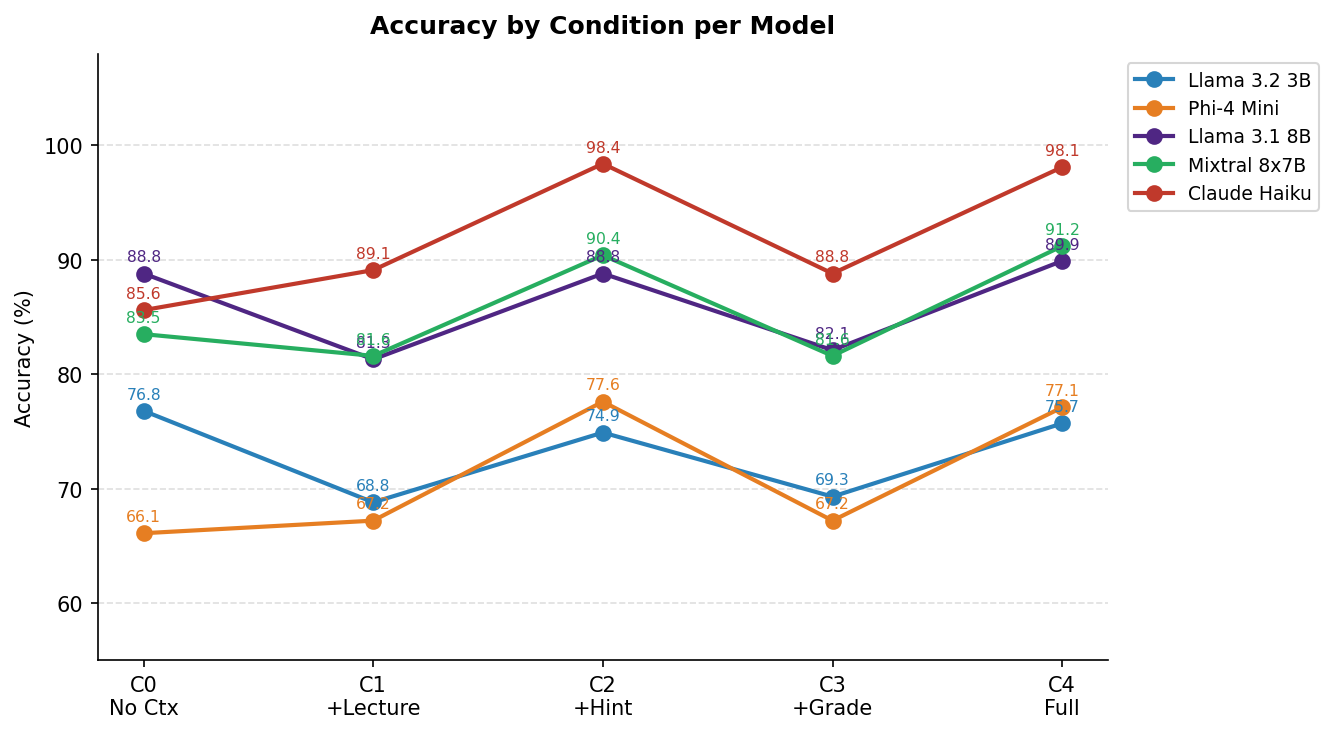
\includegraphics[width=\textwidth]{Fig/fig2_accuracy_by_condition.png}
\caption{Accuracy trajectory across conditions C0--C4 per model. The
characteristic W-shape (dip at C1, spike at C2, dip at C3, recover at C4)
confirms hints as the primary accuracy driver across all architectures.}
\label{fig:lineplot}
\end{figure*}

Fig.~\ref{fig:heatmap} reveals the dominant hint effect as a warm vertical
stripe at C2/C4 across every model, with a cool stripe at C1/C3 confirming
lecture and grade alone are insufficient for local models. Fig.~\ref{fig:lineplot}
plots the per-model trajectory: the W-shape visible for Claude Haiku and
Mixtral 8x7B confirms the hint signal as the primary driver.

\subsection{Per-Grade Accuracy}

\begin{table*}[t]
\centering
\caption{Per-Grade Accuracy (\%) for Each Model at C0, C2, and C4.
         Grade~6 is consistently the hardest; hints provide the largest grade-6 recovery.}
\label{tab:pergrade}
\renewcommand{\arraystretch}{1.3}
\begin{tabular}{lcccccccccccccccc}
\toprule
& \multicolumn{3}{c}{\textbf{Llama 3.2 3B}}
& \multicolumn{3}{c}{\textbf{Phi-4 Mini}}
& \multicolumn{3}{c}{\textbf{Llama 3.1 8B}}
& \multicolumn{3}{c}{\textbf{Mixtral 8x7B}}
& \multicolumn{3}{c}{\textbf{Claude Haiku}} \\
\cmidrule(lr){2-4}\cmidrule(lr){5-7}\cmidrule(lr){8-10}\cmidrule(lr){11-13}\cmidrule(lr){14-16}
\textbf{Grade} & C0 & C2 & C4 & C0 & C2 & C4 & C0 & C2 & C4 & C0 & C2 & C4 & C0 & C2 & C4 \\
\midrule
\rowcolor{lightpurple}
Grade 3 & 76.0 & 72.0 & 74.7 & 64.0 & 72.0 & 70.7 & 98.7 & 93.3 & 94.7 & 90.7 & 93.3 & 94.7 & 98.7 & 100.0 & 100.0 \\
Grade 4 & 86.7 & 85.3 & 85.3 & 74.7 & 85.3 & 86.7 & 94.7 & 96.0 & 96.0 & 84.0 & 88.0 & 90.7 & 97.3 & 100.0 & 100.0 \\
\rowcolor{lightpurple}
Grade 5 & 85.3 & 82.7 & 85.3 & 74.7 & 81.3 & 80.0 & 96.0 & 89.3 & 89.3 & 97.3 & 97.3 & 97.3 & 96.0 &  96.0 &  94.7 \\
Grade 6 & 64.0 & 66.7 & 64.0 & 62.7 & 80.0 & 80.0 & 73.3 & 82.7 & 85.3 & 76.0 & 89.3 & 88.0 & 64.0 &  98.7 &  98.7 \\
\rowcolor{lightpurple}
Grade 7 & 72.0 & 68.0 & 69.3 & 54.7 & 69.3 & 68.0 & 81.3 & 82.7 & 84.0 & 69.3 & 84.0 & 85.3 & 72.0 &  97.3 &  97.3 \\
\midrule
\textbf{Avg}  & 76.8 & 74.9 & 75.7 & 66.1 & 77.6 & 77.1 & 88.8 & 88.8 & 89.9 & 83.5 & 90.4 & 91.2 & 85.6 & 98.4 & 98.1 \\
\bottomrule
\end{tabular}
\end{table*}

\textbf{Grade~6 is the hardest} across all models and conditions. C0 accuracy
at grade~6 ranges from 62.7\% (Phi-4 Mini) to 76.0\% (Mixtral), well below
grades 3--5. The hint signal provides its \textbf{largest absolute recovery at
grade~6}: Claude Haiku jumps from 64.0\% to 98.7\% ($+34.7$~pp); Phi-4 Mini
from 62.7\% to 80.0\% ($+17.3$~pp); Mixtral from 76.0\% to 89.3\% ($+13.3$~pp).
Grade~6 questions have high-quality pedagogical hints that effectively constrain
the answer space when provided. Choice consistency is near-perfect for local
models ($\geq$98.9\%); Claude Haiku shows 89.9\% at C0, recovering to 100\%
under C2 and C4 where structured hints reinforce the answer format.

\subsection{Lecture Grounding and Hint Alignment}

Table~\ref{tab:grounding} reports grounding and alignment metrics averaged
across all five models for each condition.

\begin{table}[h]
\centering
\caption{Lecture Grounding (LG) and Hint Alignment (HA) Metrics, Averaged
         Across Models. Sem = cosine similarity; Ovlp = ROUGE-1 recall.}
\label{tab:grounding}
\renewcommand{\arraystretch}{1.3}
\begin{tabular}{lcccc}
\toprule
\textbf{Condition} & \textbf{LG-Sem} & \textbf{LG-Ovlp} & \textbf{HA-Sem} & \textbf{HA-Ovlp} \\
\midrule
\rowcolor{lightpurple}
C0 No Context   & 0.451 & 0.185 & 0.433 & 0.236 \\
C1 Lecture      & \textbf{0.526} & \textbf{0.314} & 0.439 & 0.263 \\
\rowcolor{lightpurple}
C2 +Hint        & 0.509 & 0.305 & \textbf{0.482} & \textbf{0.509} \\
C3 +Grade       & 0.496 & 0.290 & 0.435 & 0.245 \\
\rowcolor{lightpurple}
C4 Full Context & 0.478 & 0.280 & 0.477 & 0.450 \\
\bottomrule
\end{tabular}
\end{table}

LG-Sem and LG-Ovlp peak at C1 (0.526 and 0.314 vs.\ 0.451/0.185 at C0),
confirming models genuinely incorporate lecture language when it is provided.
However, higher grounding scores at C1 do not improve accuracy---models are
\emph{grounded but distracted}, anchoring on irrelevant lecture passages without
a hint to focus them. HA-Ovlp is the most striking signal: it remains near
0.24--0.26 for all no-hint conditions (C0, C1, C3), then more than doubles to
\textbf{0.509} at C2 and \textbf{0.450} at C4. This confirms that hints act as
an attentional anchor, and that models directly reuse hint vocabulary in their
explanations when hints are present.

\subsection{Grade Calibration}
\label{sec:calib}

Table~\ref{tab:calibration} reports FKGL and calibration error by condition,
averaged across all five models.

\begin{table}[h]
\centering
\caption{Grade Calibration by Condition, Averaged Across Models.
         FKGL = Flesch-Kincaid Grade Level of responses.
         Error $= \overline{|\text{FKGL} - \text{grade}|}$.}
\label{tab:calibration}
\renewcommand{\arraystretch}{1.3}
\begin{tabular}{lccc}
\toprule
\textbf{Condition} & \textbf{FKGL} & \textbf{Calib.\ Error} & \textbf{Resp.\ Len (w)} \\
\midrule
\rowcolor{lightpurple}
C0 No Context & 13.1 & 8.08 & 83 \\
C1 Lecture    & 13.1 & 8.12 & 93 \\
\rowcolor{lightpurple}
C2 +Hint      & 12.5 & 7.64 & 89 \\
C3 +Grade     & \textbf{10.1} & \textbf{5.17} & 92 \\
\rowcolor{lightpurple}
C4 Full       & \textbf{9.9}  & \textbf{4.90} & 83 \\
\bottomrule
\end{tabular}
\end{table}

Without grade metadata (C0--C2), all models write at FKGL 12.5--13.1
regardless of question grade (3--7). A Grade~3 student receives explanations
written at a Grade~11 reading level. With grade metadata (C3/C4), mean FKGL
drops to 9.9 and calibration error falls by \textbf{38\%} (8.08 $\to$ 4.90).

Table~\ref{tab:calib_model} shows per-model C0 vs.\ C4 calibration error.
\textbf{Phi-4 Mini} is a severe outlier: its C0 FKGL averages $\sim$18.8
(calibration error 13.8), more than twice any other model. Even with grade
conditioning its error only falls to 7.6, suggesting its reasoning-focused
pre-training~\cite{phi4} biases it toward dense academic prose that resists
grade-level adaptation. \textbf{Llama 3.1 8B} and \textbf{Claude Haiku} are
the best calibrators at C4 (mean errors 3.5 and 3.9), confirming that larger
and more instruction-tuned models adapt more effectively to grade prompts.

\begin{table}[h]
\centering
\caption{Per-Model Grade Calibration Error at C0 and C4.}
\label{tab:calib_model}
\renewcommand{\arraystretch}{1.25}
\begin{tabular}{lcccc}
\toprule
\textbf{Model} & \textbf{C0 FKGL} & \textbf{C4 FKGL} & \textbf{C0 Err} & \textbf{C4 Err} \\
\midrule
\rowcolor{lightpurple}
Claude Haiku  & 11.6 &  8.8 & 6.6 & 3.9 \\
Llama 3.1 8B  & 11.5 &  8.5 & 6.5 & 3.5 \\
\rowcolor{lightpurple}
Llama 3.2 3B  & 12.3 &  9.4 & 7.3 & 4.4 \\
Mixtral 8x7B  & 11.2 & 10.1 & 6.2 & 5.1 \\
\rowcolor{lightpurple}
Phi-4 Mini    & \textbf{18.8} & \textbf{12.6} & \textbf{13.8} & \textbf{7.6} \\
\midrule
\textbf{Average} & 13.1 & 9.9 & 8.08 & 4.90 \\
\bottomrule
\end{tabular}
\end{table}

% ─────────────────────────────────────────────────────────────────────────────
\section{Discussion}
\label{sec:discussion}

\subsection{Why Does Lecture Alone Hurt Accuracy?}

The negative C0$\to$C1 effect for most local models is the most counter-intuitive
finding. We hypothesise two mechanisms. First, \emph{context distraction}: the
lecture is 2--5 sentences of background knowledge that may not directly address
the specific question; without a hint to focus attention, the model anchors on
irrelevant phrases. Second, \emph{context interference}: the lecture may
contradict the model's parametric knowledge where training data provides a
clearer signal. Claude Haiku's positive response ($+3.5$~pp) suggests larger,
more instruction-tuned models can better integrate long-form context. The
grounding metrics confirm this: C1 achieves the highest LG-Ovlp (0.314), but
this lexical alignment with the lecture does not translate to correct answer
selection.

\subsection{Hints as the Dominant Signal}

ScienceQA pedagogical hints are authored to guide toward the key concept.
They act as an \emph{attentional cue} that collapses the answer-justification
search space, explaining why C1$\to$C2 gains ($+7$--$13$~pp) are consistently
larger and more uniform than any other condition transition. The more-than-doubling
of HA-Ovlp (0.263$\to$0.509) confirms models directly reuse hint vocabulary,
indicating genuine hint processing rather than incidental correlation.

\subsection{Grade Metadata and Language Calibration}

The negligible accuracy effect of grade metadata (RQ3) should not be interpreted
as ``grade conditioning is useless.'' The 38\% calibration error reduction
(8.08$\to$4.90) at zero accuracy cost is a strong practical argument for always
including grade metadata in K--12 LLM prompts. Phi-4 Mini's outlier behaviour
(C0 error 13.8 vs.\ next-worst 7.3) warrants particular caution: despite
grade conditioning, it writes at college-level complexity, making it unsuitable
for child-safe deployment without further fine-tuning.

\subsection{Limitations}

Only grades 3--7 are represented (dataset constraint). FKGL is a
formula-based proxy that does not capture semantic appropriateness; human
evaluation by K--12 educators would provide a stronger calibration gold
standard. The hint filter concentrates examples in Natural Science ($\sim$96\%),
precluding reliable per-subject analysis.

% ─────────────────────────────────────────────────────────────────────────────
\section{Conclusion}
\label{sec:conclusion}

We presented a five-condition ablation study on ScienceQA evaluating how
lecture context, pedagogical hints, and grade metadata affect five LLMs on
K--12 science questions. Key findings: (1) lecture context alone hurts accuracy
for most local models ($-8.0$ to $-1.9$~pp) via context distraction; (2)
pedagogical hints are the dominant signal, universally improving all five
models by $+6.1$ to $+12.8$~pp; (3) grade metadata provides negligible
accuracy change but reduces calibration error by 38\%, confirming models do
adapt language register when explicitly told the audience's grade level;
(4) Claude Haiku reaches 98.4\% with hints, while Mixtral tops local models
at 91.2\%; (5) Grade~6 is consistently the hardest grade with the largest hint
recovery; (6) Phi-4 Mini is a severe calibration outlier, writing at
college-level complexity even with grade conditioning.

For practitioners: always include pedagogical hints when available; always
include grade metadata (38\% calibration gain at zero accuracy cost); be
cautious about injecting full lecture passages without hints in smaller local
models. Future work includes extending to multimodal questions, exploring
few-shot prompting, and conducting human evaluation of grade-appropriateness
by K--12 educators.

% ─────────────────────────────────────────────────────────────────────────────
\section*{Acknowledgment}
The authors thank the communities behind Ollama, Hugging Face Datasets, and
sentence-transformers for making reproducible large-scale LLM evaluation
accessible without specialised hardware infrastructure.

% ─────────────────────────────────────────────────────────────────────────────
\bibliographystyle{IEEEtran}
\bibliography{references}

% ─────────────────────────────────────────────────────────────────────────────
\begin{IEEEbiography}[{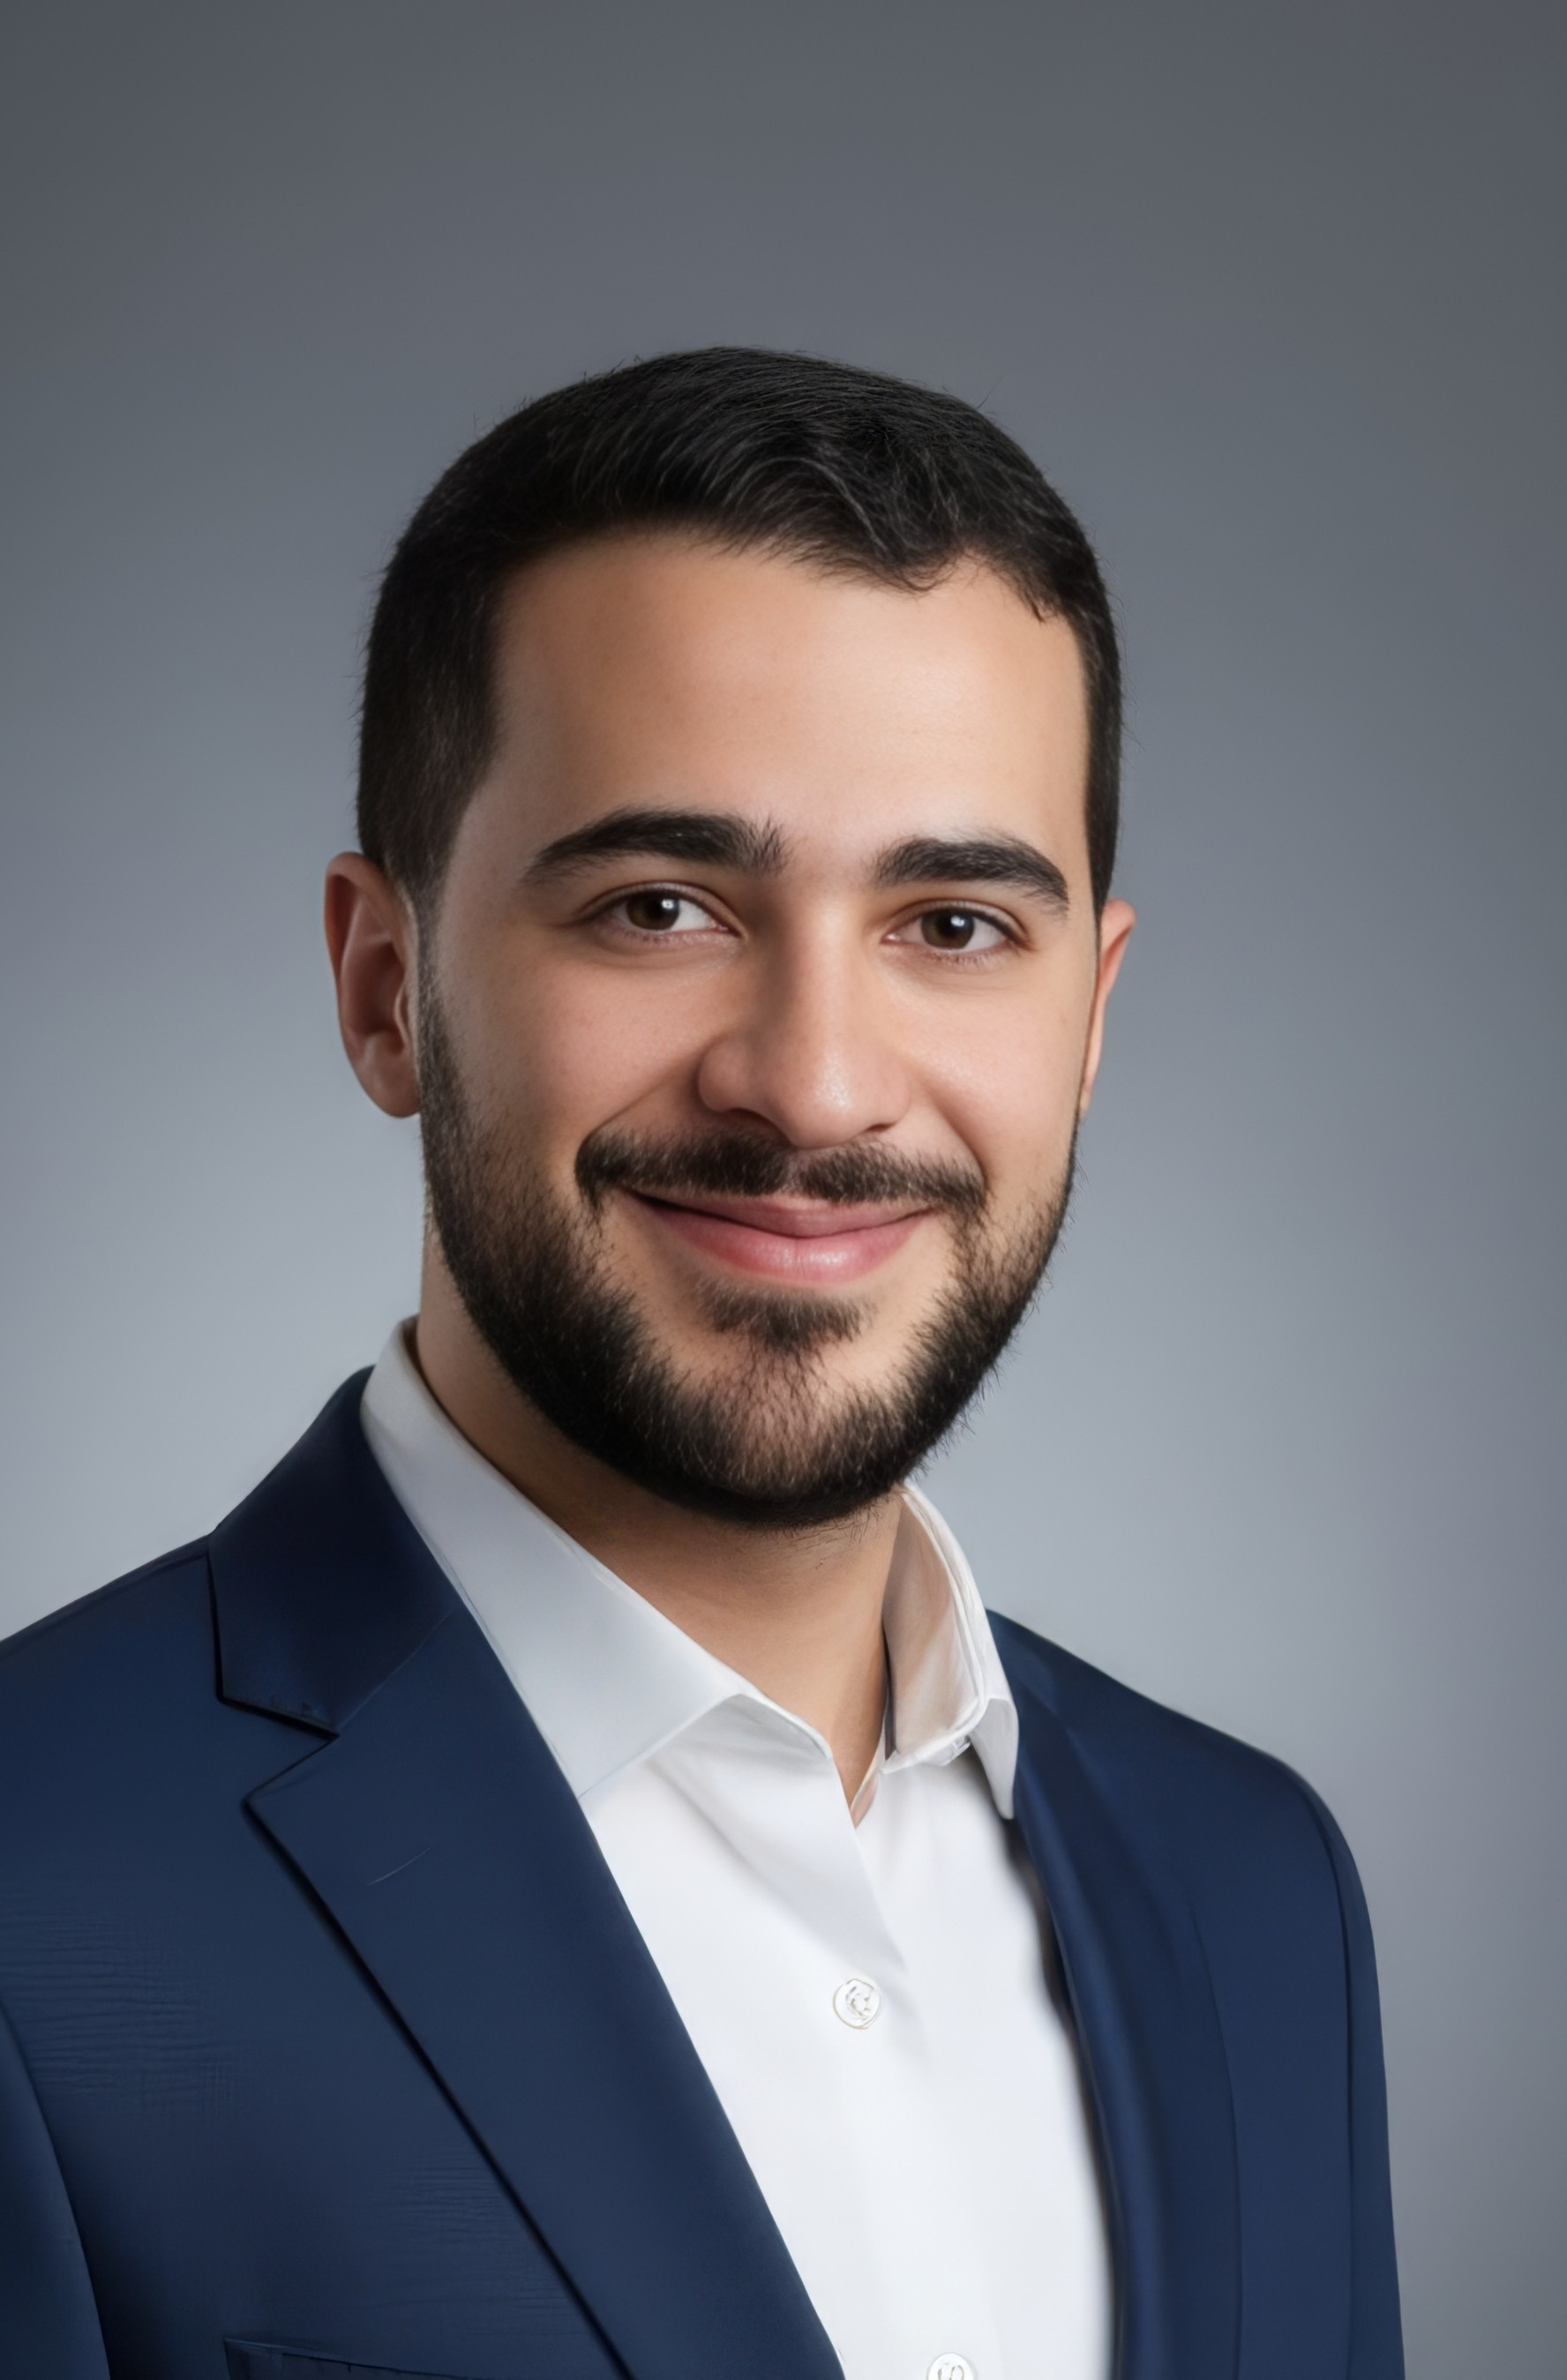
\includegraphics[width=1in,height=1.25in,clip,keepaspectratio]{Fig/Authors/1.png}}]{Ali Saab}
(Student Member, IEEE) received the B.S. degree in Computer Science from the
Lebanese University, Beirut, Lebanon, and the M.E. degree in Computer Science
from the American University of Beirut, Beirut, Lebanon. He is currently
pursuing the Ph.D. degree in Electrical and Computer Engineering at Western
University, London, ON, Canada. His research interests include large language
models, edge intelligence, explainable AI, and adaptive machine learning for
resource-constrained systems.
\end{IEEEbiography}

\begin{IEEEbiography}[{
\includegraphics[width=1in,height=1.25in,clip,keepaspectratio]{Fig/Authors/Nadine_Charaf.jpg}}]{Nadine Charaf}
(Student Member, IEEE) received the B.S. degree in Applied Mathematics with a
Minor in Computer Science, with High Distinction, from the American University
of Beirut, Beirut, Lebanon, in 2023. She is currently pursuing the Ph.D. degree
in Electrical and Computer Engineering at Western University, London, ON, Canada.
Her research interests include quantum machine learning, optimisation, and
AI-driven educational systems.
\end{IEEEbiography}

\end{document}
